\section{Experiment I: Baseline}
We first compare the LSTM models against a baseline MLP on the relatively easy task of non-novel speakers. Meaning, we group the data set such that, for a particular speaker, it is possible for some of their syllables to appear in the training set, while others are in the test set. Specifically, we randomly assign each example in the data set to the training, testing, and validation sets with a ratio of 2:1:1. 

We employ the accuracy, precision, and recall \cite{torgo2009precision} as metrics to judge the performance of each model. Precision and recall are considered due to the medical nature of these experiments. That is, most people do not suffer from dysarthria, but it is the instances in which one does that are important to classify correctly. We therefore define a metric to measure the chance that a dysarthria patient will receive a negative result $FN = 1 - recall$. In an analogous fashion, we define a metric for false-positives $FP = 1 - precision$. Because individuals who receive a negative prediction (i.e., they do not suffer from dysarthria) are less likely to seek a second opinion, we are especially interested in the minimization of $FN$. 

\begin{table}[h]
\centering
\caption{Experimental results}
\begin{tabular}{|l|c|c|c|}
\hline
\multicolumn{1}{|c|}{}    &   Accuracy     &   FP         &     FN         \\ \hline
Baseline                    &   80.1\%     &   -          &     -           \\ \hline
LSTM-1                      &   88.7\%     &   11.5\%     &     8.8\%       \\ \hline
LSTM-2                      &   88.7\%     &   12.0\%     &     8.3\%       \\ \hline
Bi-LSTM-1                   &   87.8\%     &   13.4\%     &     8.2\%      \\ \hline
\end{tabular}
\label{tab-exp-1-results}
\end{table}

Table \ref{tab-exp-1-results} depicts the results for each experiment. Given that the majority classifier would achieve an accuracy of about $53\%$, the baseline is a significant improvement. Moreover, LSTM-1 and LSTM-2 achieve similar performance, beating the baseline and making a marginal improvement upon the Bi-LSTM-1 model.

\begin{figure}[h]
\centering
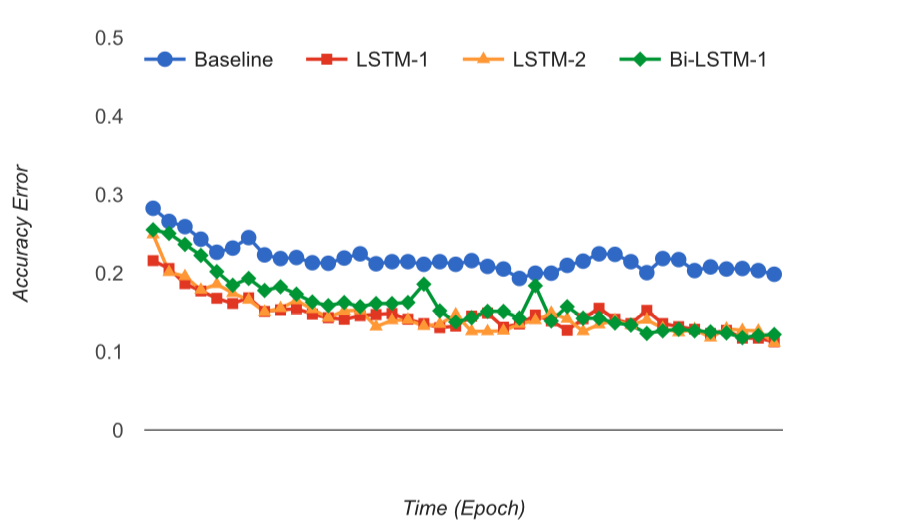
\includegraphics[width=\columnwidth]{convergence}
\caption{Error rate over the 40 epochs of training. The three LSTM models start training with slightly different error rates, but all  eventually converge to a rate superior to the baseline. }
\label{fig-convergence}
\end{figure}

Figure \ref{fig-convergence} shows the accuracy convergence of each model. The LSTM's clearly outperform the baseline; however, increasing the expressive capacity through adding layers and passes over the data did not result in significant performance improvements. LSTM-1 and LSTM-2 achieved the same accuracy, with the latter improving upon the false negatives metric. Because adding a layer resulted in the same performance, and adding another pass was slightly detrimental, we did not consider a two-layer bidirectional model. 

LSTM-2's $88.7$\% accuracy and 8.2\% false negative rate constitute a promising attempt at classifying dysarthria among both afflicted and healthy speakers, but it is important to remember the practical application of these models. When such a system attempts to classify an individual, it has likely never been trained on any of their data. While it is clear that the LSTM models outperform the baseline, we are more interested in how they perform when evaluating novel speakers. 